\documentclass[ucs,10pt]{beamer}
% Template for talks using the Logo of STCE and Corporate Design of RWTH Aachen
% adapted from:
% https://www.mi.fu-berlin.de/w/Mi/BeamerTemplateCorporateDesign

\usepackage{amsmath,dsfont,listings}

%%% STCE logo
% small version for upper right corner of normal pages
\pgfdeclareimage[height=0.9cm]{university-logo}{rwth_i12_softw-werkz_en_rgb.png}
\logo{\pgfuseimage{university-logo}}
% large version for upper right corner of title page
\pgfdeclareimage[height=1cm]{big-university-logo}{rwth_i12_softw-werkz_en_rgb.png}
\newcommand{\titleimage}[1]{\pgfdeclareimage[height=2cm]{title-image}{#1}}
\titlegraphic{\pgfuseimage{title-image}}
%%% end STCE logo

% NOTE: 1cm = 0.393 in = 28.346 pt;    1 pt = 1/72 in = 0.0352 cm
\setbeamersize{text margin right=3.5mm, text margin left=7.5mm}  % text margin

% colors to be used
\definecolor{text-grey}{RGB}{51, 51, 51} % grey text on white background
\definecolor{bg-grey}{rgb}{0.66, 0.65, 0.60} % grey background (for white text)
\definecolor{rwth-blue}{RGB}{0, 83, 159} % blue text
\definecolor{rwth-green}{RGB}{153, 204, 0} % green text
\definecolor{rwth-red}{RGB}{204, 0, 0} % red text (used by \alert)

% switch off the sidebars
% TODO: loading \useoutertheme{sidebar} (which is maybe wanted) also inserts
%   a sidebar on title page (unwanted), also indents the page title (unwanted?),
%   and duplicates the navigation symbols (unwanted)
\setbeamersize{sidebar width left=0cm, sidebar width right=0mm}
\setbeamertemplate{sidebar right}{}
\setbeamertemplate{sidebar left}{}
%    XOR
% \useoutertheme{sidebar}

% frame title
% is truncated before logo and splits on two lines
% if neccessary (or manually using \\)
\setbeamertemplate{frametitle}{%
    \vskip-30pt \color{purple}\large%
    \begin{minipage}[b][23pt]{80.5mm}%
    \flushleft\insertframetitle%
    \end{minipage}%
}

%%% title page
% TODO: get rid of the navigation symbols on the title page.
%   actually, \frame[plain] *should* remove them...
\setbeamertemplate{title page}{
% upper right: STCE logo
\vskip2pt\hfill\pgfuseimage{big-university-logo} \\
\vskip6pt\hskip3pt
% title image of the presentation
% set the title and the author
\begin{center}
\vskip4pt
\large \inserttitle \vskip5pt  \small \insertsubtitle
\vskip8pt
	\normalsize \insertauthor %\\ 
	%\includegraphics[width=2cm]{../../foto_naumann}	
\\ [5mm]
	\footnotesize \insertinstitute 
\end{center}
}
%%% end title page

%%% colors
\usecolortheme{lily}
\setbeamercolor*{normal text}{fg=black,bg=white}
\setbeamercolor*{alerted text}{fg=rwth-red}
\setbeamercolor*{example text}{fg=rwth-green}
\setbeamercolor*{structure}{fg=rwth-blue}

\setbeamercolor*{block title}{fg=white,bg=black!50}
\setbeamercolor*{block title alerted}{fg=white,bg=black!50}
\setbeamercolor*{block title example}{fg=white,bg=black!50}

\setbeamercolor*{block body}{bg=black!10}
\setbeamercolor*{block body alerted}{bg=black!10}
\setbeamercolor*{block body example}{bg=black!10}

\setbeamercolor{bibliography entry author}{fg=rwth-blue}
% TODO: this doesn't work at all:
\setbeamercolor{bibliography entry journal}{fg=text-grey}

\setbeamercolor{item}{fg=rwth-blue}
\setbeamercolor{navigation symbols}{fg=text-grey,bg=bg-grey}
%%% end colors

%%% headline
\setbeamertemplate{headline}{
\vskip4pt\hfill\insertlogo\hspace{3.5mm} % logo on the right

\vskip6pt\color{rwth-blue}\rule{\textwidth}{0.4pt} % horizontal line
}
%%% end headline

%%% footline
\newcommand{\footlinetext}{\insertshortinstitute, \insertshorttitle}
\setbeamertemplate{footline}{
\vskip5pt\color{rwth-blue}\rule{\textwidth}{0.4pt}\\ % horizontal line
\vskip2pt
\makebox[123mm]{\hspace{7.5mm}
\color{rwth-blue}\footlinetext
\hfill \raisebox{-1pt}{\usebeamertemplate***{navigation symbols}}
\hfill \insertframenumber}
\vskip4pt
}
%%% end footline

%%% settings for listings package
\lstset{extendedchars=true, showstringspaces=false, basicstyle=\footnotesize\sffamily, tabsize=2, breaklines=true, breakindent=10pt, frame=l, columns=fullflexible}
\lstset{language=C++} % this sets the syntax highlighting
\lstset{mathescape=true} % this switches on $...$ substitution in code
% enables UTF-8 in source code:
\lstset{literate={ä}{{\"a}}1 {ö}{{\"o}}1 {ü}{{\"u}}1 {Ä}{{\"A}}1 {Ö}{{\"O}}1 {Ü}{{\"U}}1 {ß}{\ss}1}
%%% end listings
  
\usepackage{multicol}
\usepackage{caption}
\usepackage{subcaption}

\begin{document}
\title[{\tt info@stce.rwth-aachen.de}]{\textcolor{rwth-blue}{Software Lab Computational Engineering Science} \vspace{.2cm} \\ {\small Group 12, Pusher Mechanism}}
\author[Group 12, Pusher Mechanism]{Aaron Floerke, Arseniy Kholod, Xinyang Song and Yanliang Zhu} 
\institute[Software Lab CES]{
{Informatik 12: Software and Tools for Computational Engineering (STCE)} \\ RWTH Aachen University \vspace{.5cm}
}
\date[]{}

\begin{frame}[plain]
\titlepage
\end{frame}

\begin{frame}
	\frametitle{Contents}
\tableofcontents
\end{frame}

\section{Preface}

\begin{frame}
\frametitle{Preface \\
	\small \color{rwth-blue} Four-bar linkage model}
	\begin{center}
		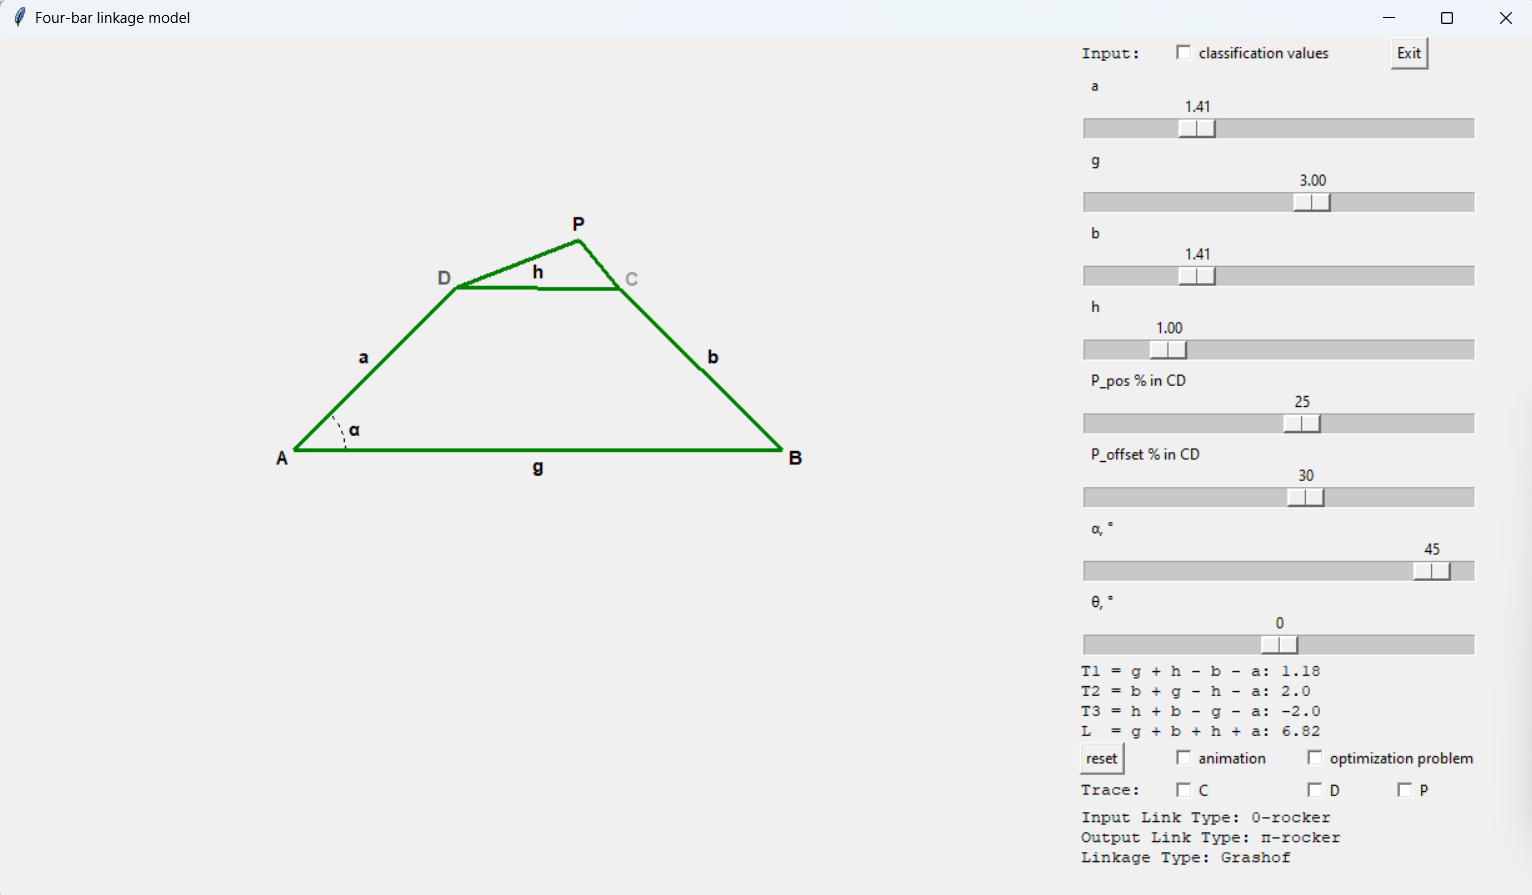
\includegraphics[width=\linewidth]{./Figures/GUI_screen.png}
	\end{center}
\end{frame}

\section{Analysis}

\subsection{User Requirements}

\begin{frame}
\frametitle{Analysis \\
	\small \color{rwth-blue} User Requirements}
	  \begin{minipage}{\linewidth}
		\centering
		\begin{minipage}{0.6\linewidth}
			\begin{itemize}
				\item Implement 27 motion types of the four-bar linkage with one bar fixed:
				\begin{itemize}
					\item Classification values:
					\begin{itemize}
						\item $T_1 = g + h - b - a$
						\item $T_2 = b + g - h - a$
						\item $T_3 = h + b - g - a$
					\end{itemize}
				\end{itemize}
				\item Implement GUI with motion animation and the ability to choose geometrical parameters:
				\begin{itemize}
					\item Length of the bars
					\item Position of the coupler
					\item Input angle
					\item Angle relative to the horizon
					\item Classification values as alternative input
				\end{itemize}
			\end{itemize}
		\end{minipage}
		\hspace{0.05\linewidth}
		\begin{minipage}{0.31\linewidth}
			\begin{figure}[h]
				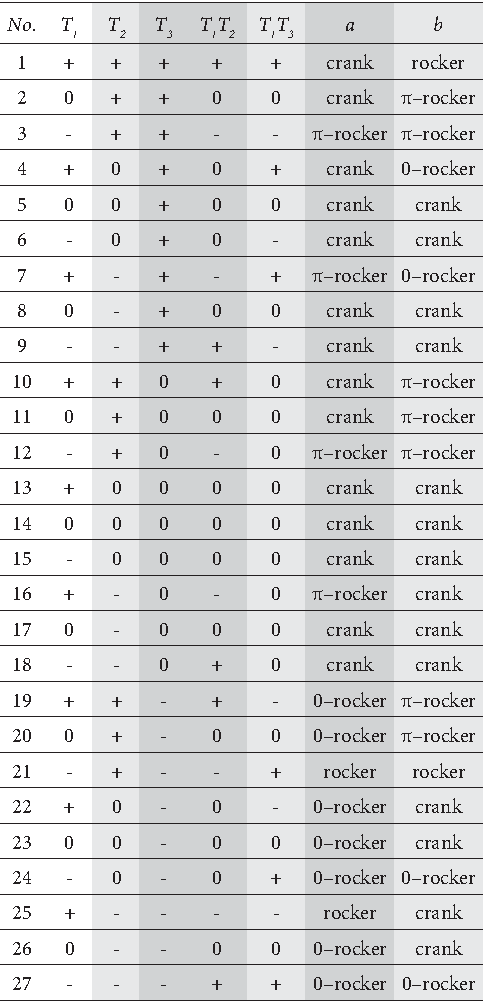
\includegraphics[width=\textwidth]{./Figures/motion_classification.pdf}
			\end{figure}
		\end{minipage}
	\end{minipage}
	{\tiny Figure from "Classification, geometrical and kinematic analysis of four-bar linkages" 10.15308/Sinteza-2018-261-266 by Ivana Cvetkovic et al.}
\end{frame}

\begin{frame}
\frametitle{Analysis \\
	\small \color{rwth-blue} User Requirements}
	\begin{center}
		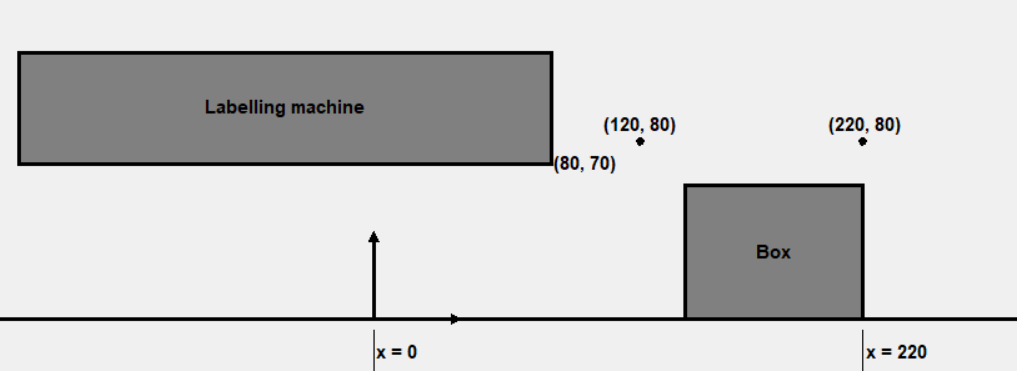
\includegraphics[width=0.75\linewidth]{./Figures/optimization_problem.png}
	\end{center}
	\begin{itemize}
			\item Solve an optimization problem:
			\begin{itemize}
				\item Push box with size $80\times60$ from $x=220$ to $x=0$
				\item Do not cross the area of the labelling machine (Area with $x<80$ and $y>70$).
				\item Pass above points $(120, 80)$ and $(220, 80)$
			\end{itemize}
	\end{itemize}
\end{frame}


\subsection{System Requirements}

\begin{frame}
	\frametitle{System Requirements \\
		\small \color{rwth-blue} Functional}
	\begin{itemize}
		\item \textbf{Four-bar linkage model}:
		\begin{itemize}
			\item System simulates all the motion types of the four-bar linkage.
			\item System does not crash with any input of geometrical configuration.
		\end{itemize}
		\item \textbf{Tests}:
		\begin{itemize}
			\item Implement test cases for geometry.
			\item Implement test cases with bad input to test system stability.
		\end{itemize}
		
		\item \textbf{Graphical User Interface}:
		\begin{itemize}
			\item GUI provides the four-bar linkage visualization and motion animation.
			\item User can input geometrical data by moving a point on a slide bar.
			\item GUI is coupled with the four-bar linkage model to use implemented motion cases for animation.
			\item GUI provides tracing for trajectories of the points.
			\item GUI classifies of the linkage.
		\end{itemize}
		\item \textbf{Optimization problem}:
		\begin{itemize}
			\item It should be possible to find a solution (manually) for the optimization problem using the four-bar linkage model.
			\item GUI visualizes the solution.
		\end{itemize}
	\end{itemize}
\end{frame}

\begin{frame}
	\frametitle{System Requirements \\
		\small \color{rwth-blue} Non-Functional}
	\begin{itemize}
		\item \textbf{Performance}:
		\begin{itemize}
			\item The four-bar linkage model is fast enough to provide smooth GUI animations.
			\item GUI animations are not slower than 30 frames per second.
		\end{itemize}
		\item \textbf{Usability}:
		\begin{itemize}
			\item Every essential part of the four-bar linkage model is well documented.
			\item GUI is easy to operate and all functionalities are self-explanatory.
			\item GUI source code is well documented.
		\end{itemize}
	\end{itemize}
\end{frame}

\section{Design}

\subsection{System Requirements}

\begin{frame}
\frametitle{Design \\
	\small \color{rwth-blue} Principal Components and Third-Party Software}
\end{frame}

\subsection{Class Model(s)}

\begin{frame}
\frametitle{Design \\
	\small \color{rwth-blue} Class Model(s)}
\end{frame}

\section{Implementation}

\subsection{Development Infrastructure}

\begin{frame}
\frametitle{Implementation \\
	\small \color{rwth-blue} Development Infrastructure}
\end{frame}

\subsection{Four-Bar Linkage Model}

\begin{frame}
\frametitle{Implementation \\
	\small \color{rwth-blue} Four-Bar Linkage Model}
\end{frame}

\subsection{Software Tests}

\begin{frame}
	\frametitle{Implementation \\
		\small \color{rwth-blue} Software Tests}
\end{frame}

\subsection{GUI}

\begin{frame}
\frametitle{Implementation \\
	\small \color{rwth-blue} GUI}
\end{frame}

\section{Results}

\subsection{27 movement types}

\begin{frame}
\frametitle{Results \\
	\small \color{rwth-blue} 27 movement types}	
	\begin{center}
		\begin{tabular}{ c@{\hskip 5pt}c@{\hskip 5pt}c@{\hskip 5pt}c@{\hskip 5pt}c}
			\begin{minipage}{0.185\linewidth}\begin{center} 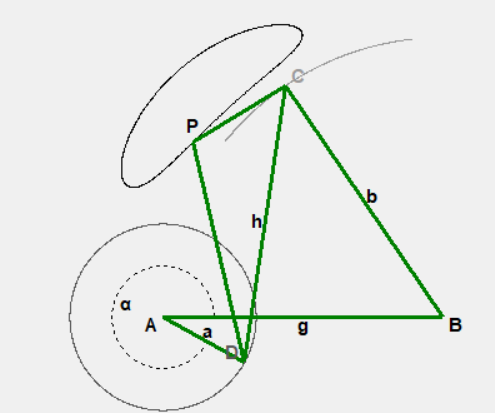
\includegraphics[width=\linewidth]{./Figures/27_motion_cases/111.png} \hfill {\tiny $T_{1,2,3} = 1.0, 1.0, 1.0$}\end{center}\end{minipage}& \begin{minipage}{0.185\linewidth}\begin{center} 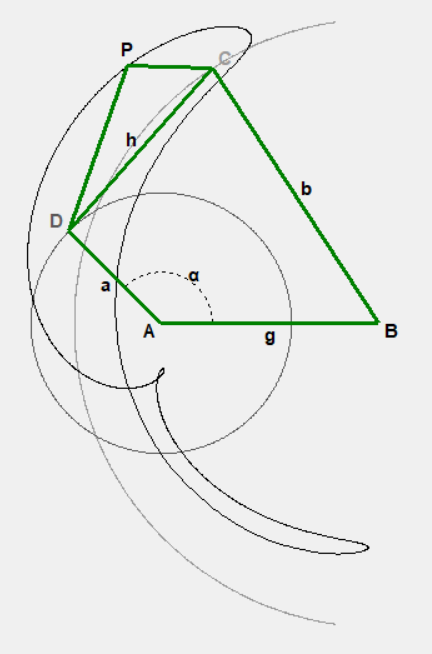
\includegraphics[width=0.55\linewidth]{./Figures/27_motion_cases/011.png} \hfill {\tiny $T_{1,2,3} = 0.0, 1.0, 1.0$}\end{center}\end{minipage}& \begin{minipage}{0.185\linewidth}\begin{center} 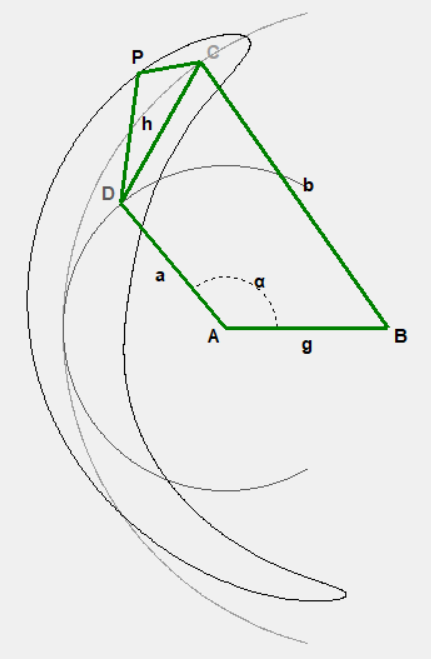
\includegraphics[width=0.55\linewidth]{./Figures/27_motion_cases/-111.png} \hfill {\tiny $T_{1,2,3} = -1.0, 1.0, 1.0$}\end{center}\end{minipage}& \begin{minipage}{0.185\linewidth}\begin{center} 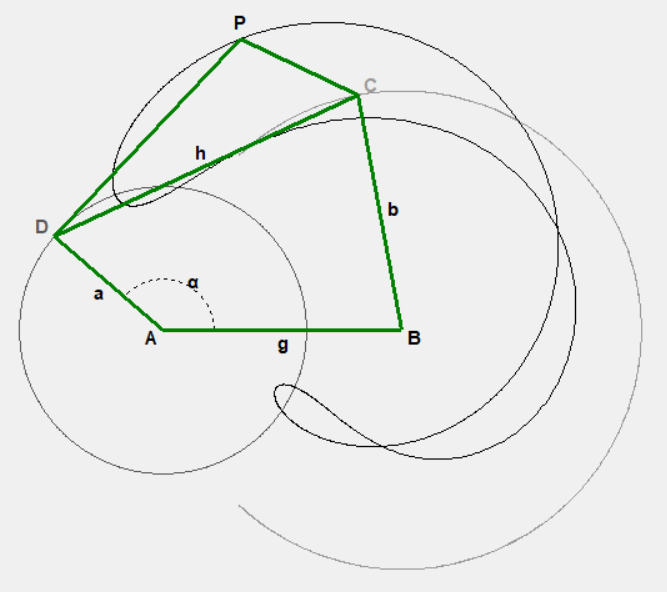
\includegraphics[width=\linewidth]{./Figures/27_motion_cases/101.png} \hfill {\tiny $T_{1,2,3} = 1.0, 0.0, 1.0$}\end{center}\end{minipage}& \begin{minipage}{0.185\linewidth}\begin{center} 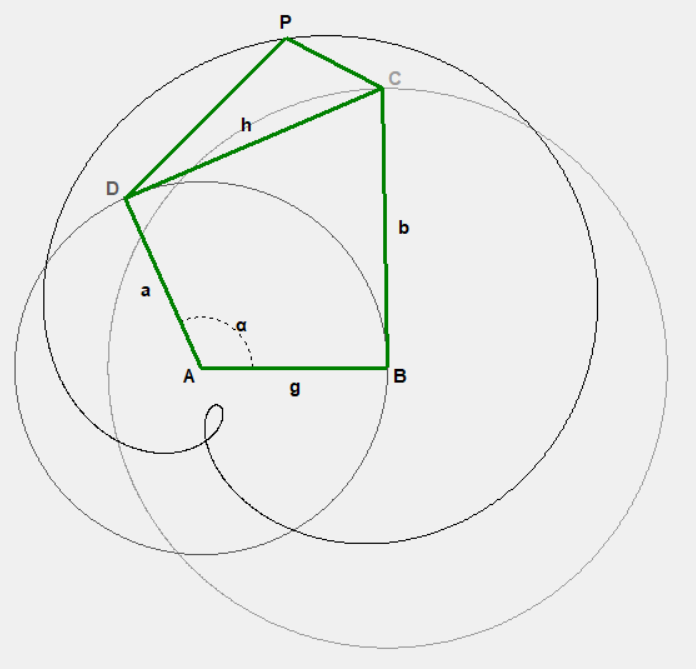
\includegraphics[width=0.9\linewidth]{./Figures/27_motion_cases/001.png} \hfill {\tiny $T_{1,2,3} = 0.0, 0.0, 1.0$}\end{center}\end{minipage} \\
			\begin{minipage}{0.185\linewidth}\begin{center} 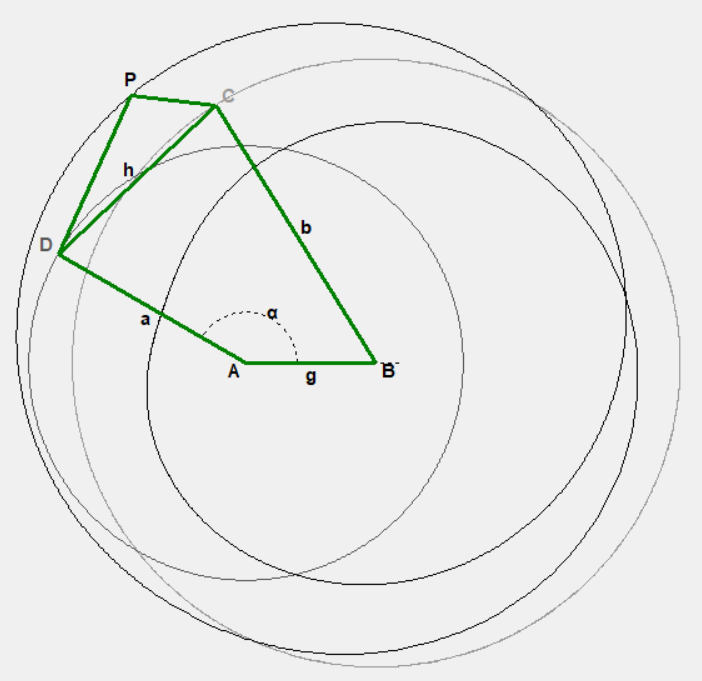
\includegraphics[width=0.8\linewidth]{./Figures/27_motion_cases/-101.png} \hfill {\tiny $T_{1,2,3} = -1.0, 0.0, 1.0$}\end{center}\end{minipage}& \begin{minipage}{0.185\linewidth}\begin{center} 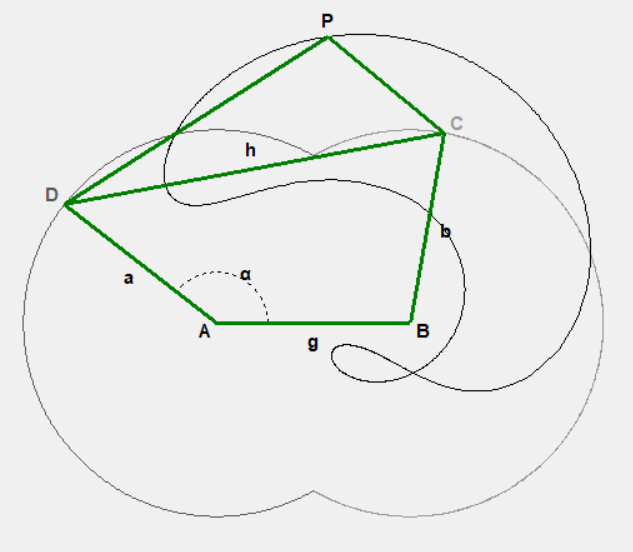
\includegraphics[width=0.9\linewidth]{./Figures/27_motion_cases/1-11.png} \hfill {\tiny $T_{1,2,3} = 1.0, -1.0, 1.0$}\end{center}\end{minipage}& \begin{minipage}{0.185\linewidth}\begin{center} 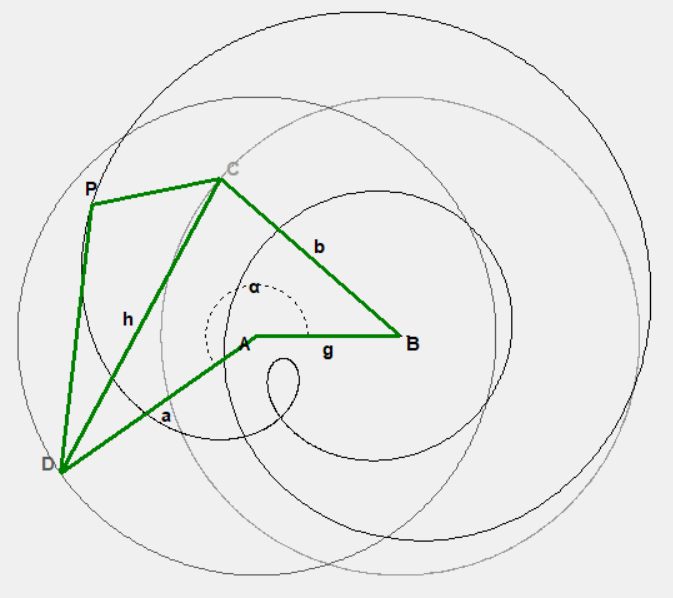
\includegraphics[width=0.9\linewidth]{./Figures/27_motion_cases/0-11.png} \hfill {\tiny $T_{1,2,3} = 0.0, -1.0, 1.0$}\end{center}\end{minipage}& \begin{minipage}{0.2\linewidth}\begin{center} 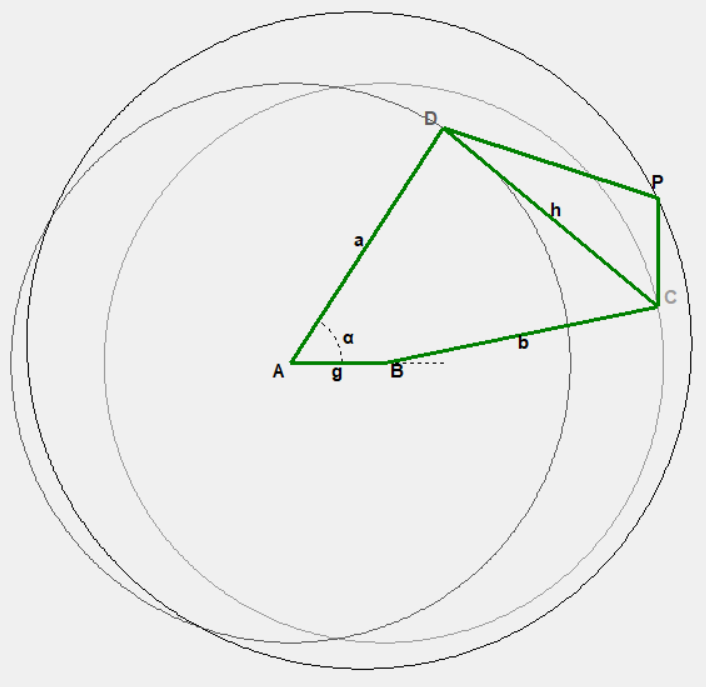
\includegraphics[width=0.75\linewidth]{./Figures/27_motion_cases/-1-11.png} \hfill {\tiny $T_{1,2,3} = -1.0, -1.0, 1.0$}\end{center}\end{minipage}& \begin{minipage}{0.185\linewidth}\begin{center} 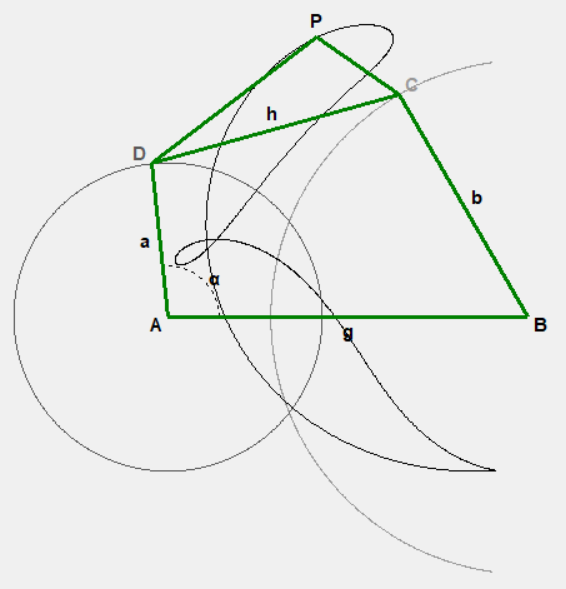
\includegraphics[width=0.75\linewidth]{./Figures/27_motion_cases/110.png} \hfill {\tiny $T_{1,2,3} = 1.0, 1.0, 0.0$}\end{center}\end{minipage} \\
			\begin{minipage}{0.185\linewidth}\begin{center} 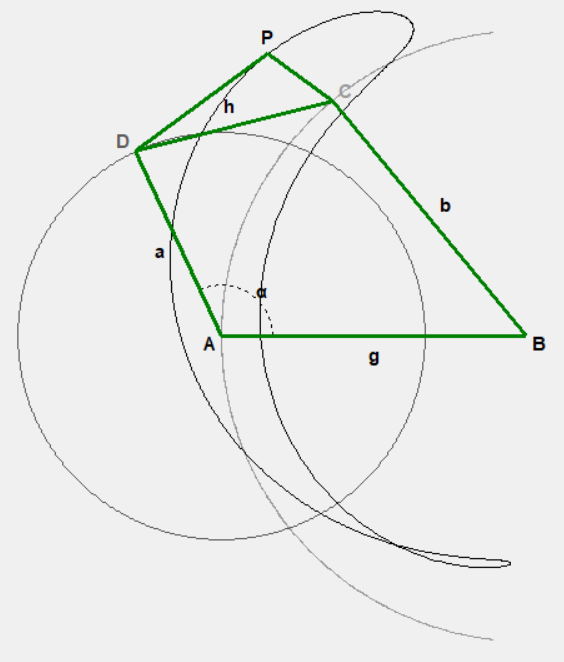
\includegraphics[width=0.65\linewidth]{./Figures/27_motion_cases/010.png} \hfill {\tiny $T_{1,2,3} = 0.0, 1.0, 0.0$}\end{center}\end{minipage}& \begin{minipage}{0.185\linewidth}\begin{center} 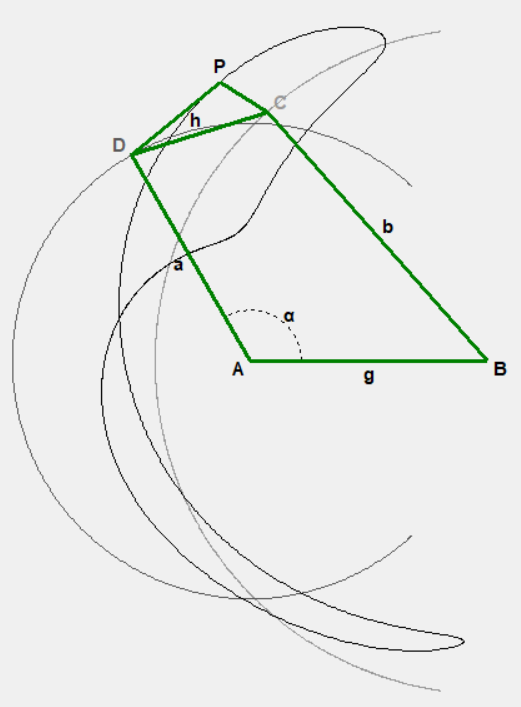
\includegraphics[width=0.55\linewidth]{./Figures/27_motion_cases/-110.png} \hfill {\tiny $T_{1,2,3} = -1.0, 1.0, 0.0$}\end{center}\end{minipage}& \begin{minipage}{0.185\linewidth}\begin{center} 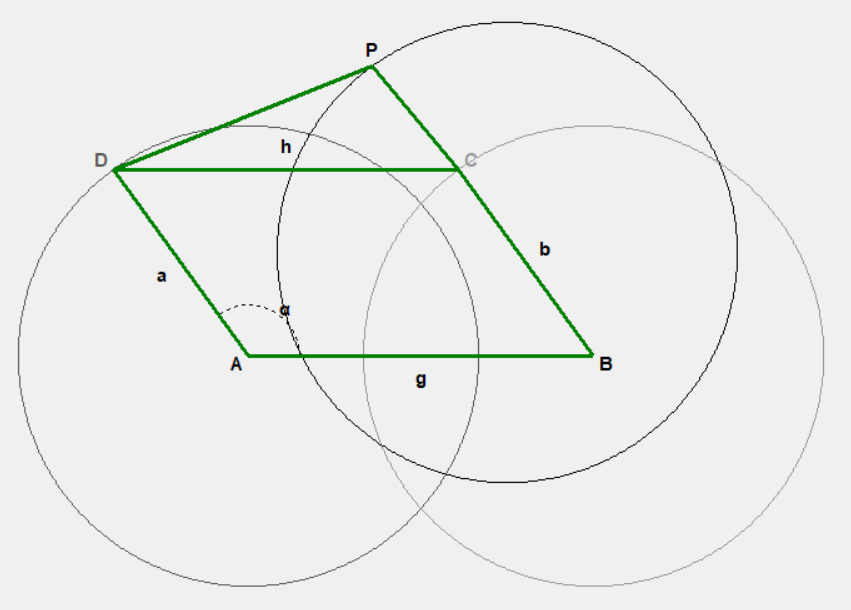
\includegraphics[width=\linewidth]{./Figures/27_motion_cases/100.png} \hfill {\tiny $T_{1,2,3} = 1.0, 0.0, 0.0$}\end{center}\end{minipage}& \begin{minipage}{0.185\linewidth}\begin{center} 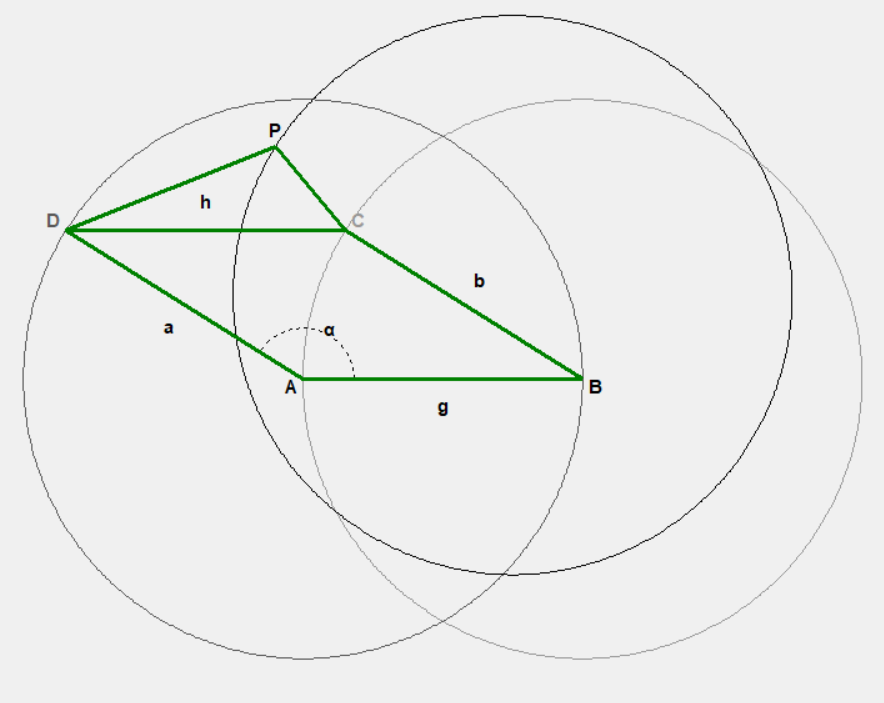
\includegraphics[width=0.9\linewidth]{./Figures/27_motion_cases/000.png} \hfill {\tiny $T_{1,2,3} = 0.0, 0.0, 0.0$}\end{center}\end{minipage}& \begin{minipage}{0.185\linewidth}\begin{center} 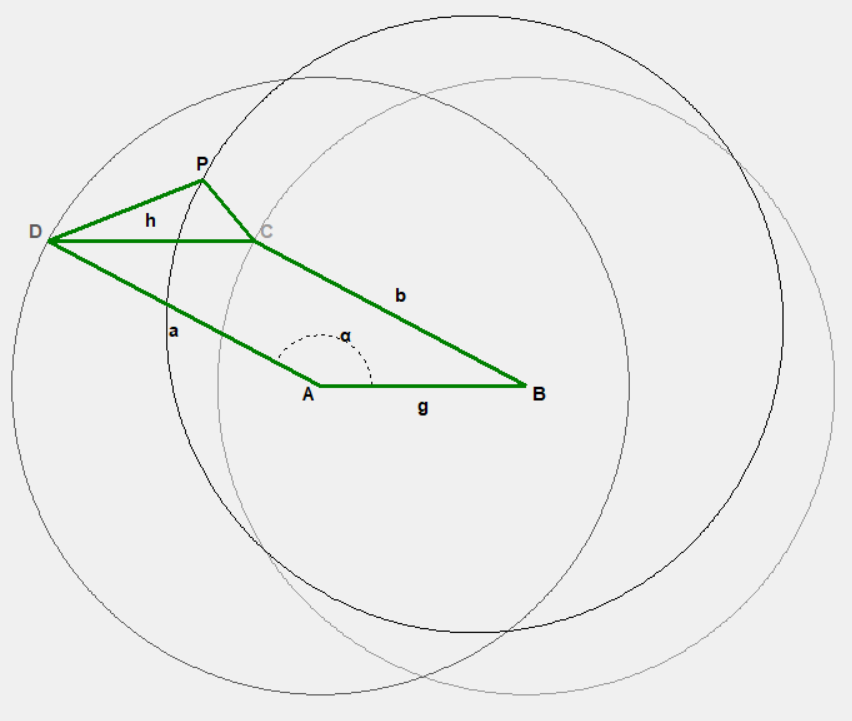
\includegraphics[width=0.8\linewidth]{./Figures/27_motion_cases/-100.png} \hfill {\tiny $T_{1,2,3} = -1.0, 0.0, 0.0$}\end{center}\end{minipage} \\
		\end{tabular}
	\end{center}
\end{frame}

\begin{frame}
\frametitle{Results \\
	\small \color{rwth-blue} 27 movement types}	
\begin{center}
	\begin{tabular}{ c@{\hskip 5pt}c@{\hskip 5pt}c@{\hskip 5pt}c}
		\begin{minipage}{0.185\linewidth}\begin{center} 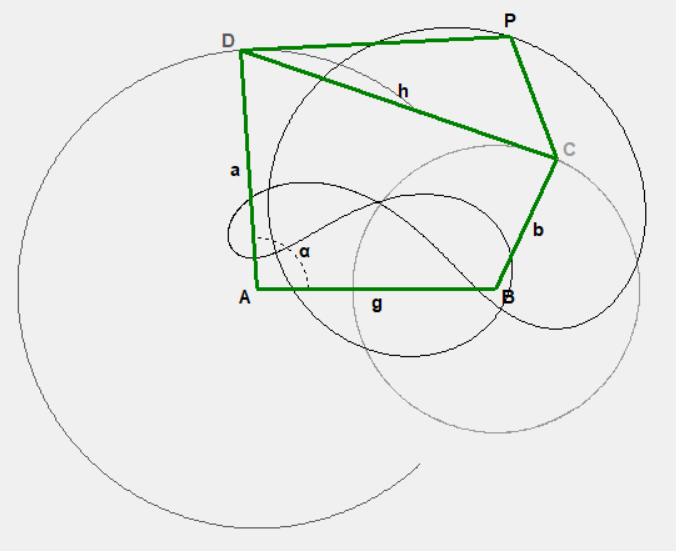
\includegraphics[width=0.9\linewidth]{./Figures/27_motion_cases/1-10.png} \hfill {\tiny $T_{1,2,3} = 1.0, -1.0, 0.0$}\end{center}\end{minipage}& \begin{minipage}{0.185\linewidth}\begin{center} 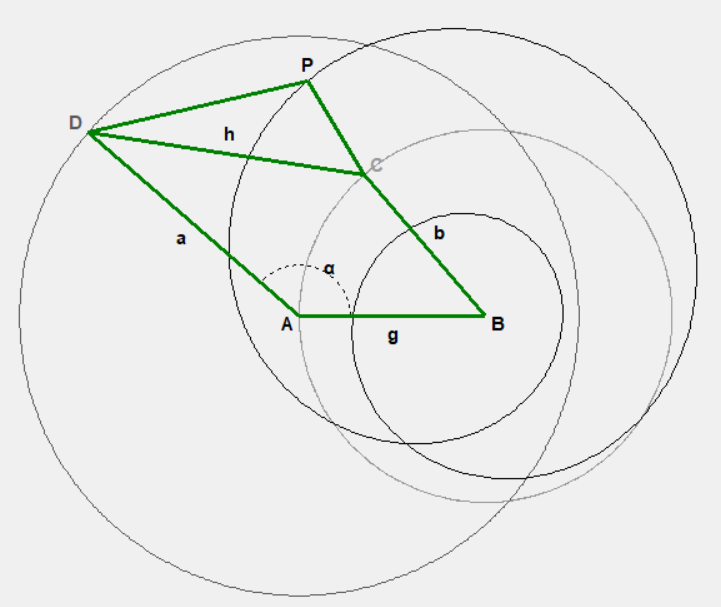
\includegraphics[width=0.85\linewidth]{./Figures/27_motion_cases/0-10.png} \hfill {\tiny $T_{1,2,3} = 0.0, -1.0, 0.0$}\end{center}\end{minipage}& \begin{minipage}{0.21\linewidth}\begin{center} 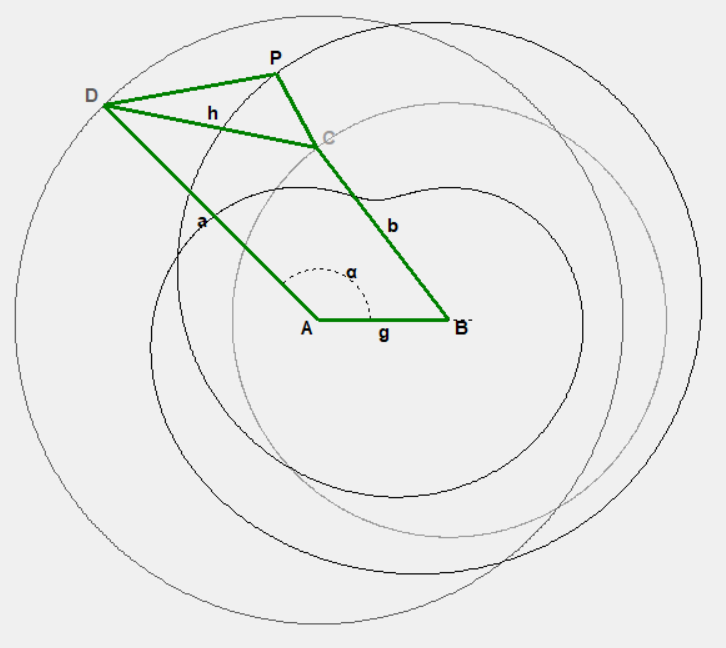
\includegraphics[width=0.7\linewidth]{./Figures/27_motion_cases/-1-10.png} \hfill {\tiny $T_{1,2,3} = -1.0, -1.0, 0.0$}\end{center}\end{minipage}& \begin{minipage}{0.185\linewidth}\begin{center} 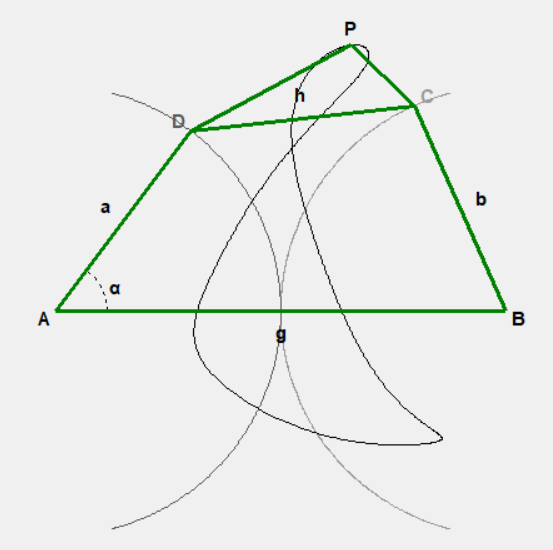
\includegraphics[width=0.7\linewidth]{./Figures/27_motion_cases/11-1.png} \hfill {\tiny $T_{1,2,3} = 1.0, 1.0, -1.0$}\end{center}\end{minipage} \\ \begin{minipage}{0.185\linewidth}\begin{center} 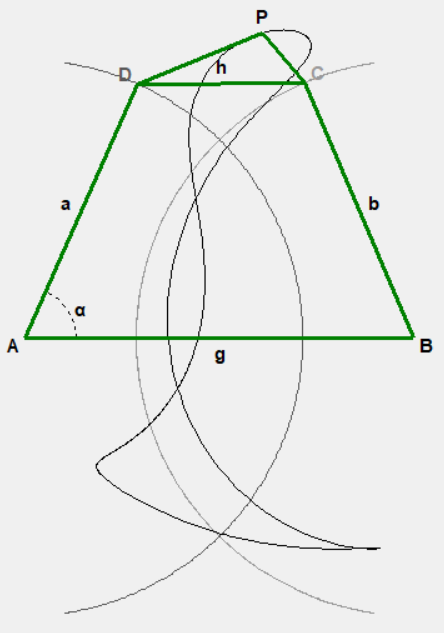
\includegraphics[width=0.65\linewidth]{./Figures/27_motion_cases/01-1.png} \hfill {\tiny $T_{1,2,3} = 0.0, 1.0, -1.0$}\end{center}\end{minipage}&
		\begin{minipage}{0.21\linewidth}\begin{center} 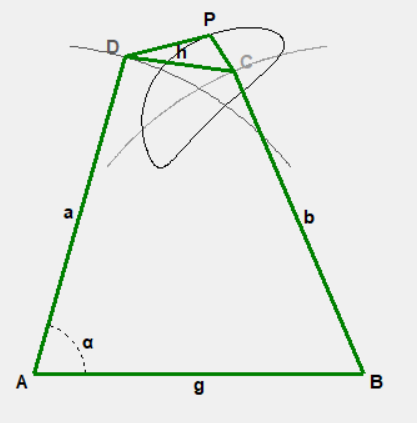
\includegraphics[width=0.75\linewidth]{./Figures/27_motion_cases/-11-1.png} \hfill {\tiny $T_{1,2,3} = -1.0, 1.0, -1.0$}\end{center}\end{minipage}& \begin{minipage}{0.185\linewidth}\begin{center} 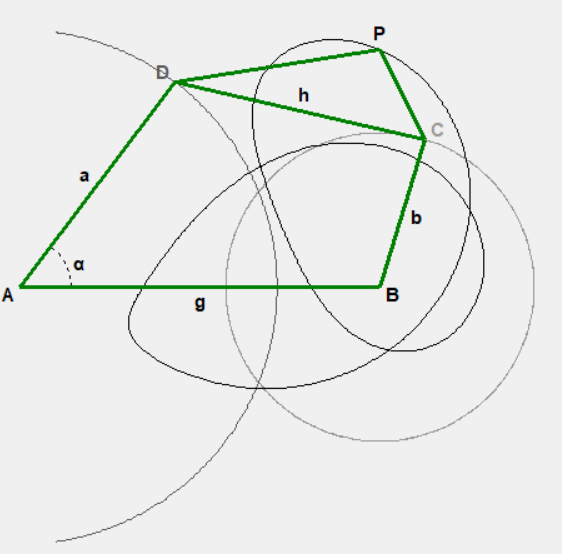
\includegraphics[width=0.85\linewidth]{./Figures/27_motion_cases/10-1.png} \hfill {\tiny $T_{1,2,3} = 1.0, 0.0, -1.0$}\end{center}\end{minipage}& \begin{minipage}{0.185\linewidth}\begin{center} 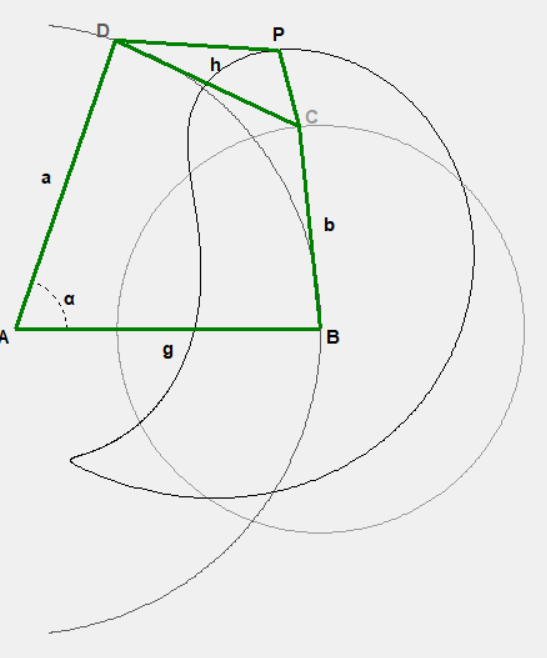
\includegraphics[width=0.7\linewidth]{./Figures/27_motion_cases/00-1.png} \hfill {\tiny $T_{1,2,3} = 0.0, 0.0, -1.0$}\end{center}\end{minipage} \\ \begin{minipage}{0.2\linewidth}\begin{center} 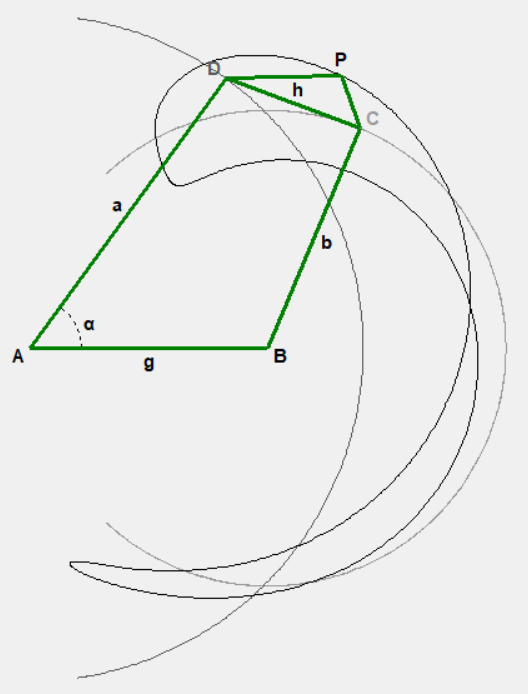
\includegraphics[width=0.7\linewidth]{./Figures/27_motion_cases/-10-1.png} \hfill {\tiny $T_{1,2,3} = -1.0, 0.0, -1.0$}\end{center}\end{minipage}& \begin{minipage}{0.21\linewidth}\begin{center} 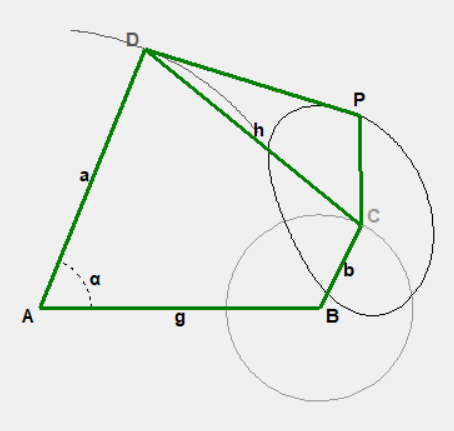
\includegraphics[width=0.9\linewidth]{./Figures/27_motion_cases/1-1-1.png} \hfill {\tiny $T_{1,2,3} = 1.0, -1.0, -1.0$}\end{center}\end{minipage}&
		\begin{minipage}{0.21\linewidth}\begin{center} 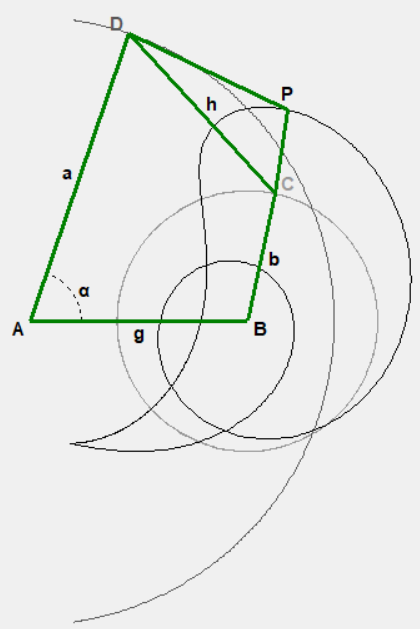
\includegraphics[width=0.55\linewidth]{./Figures/27_motion_cases/0-1-1.png} \hfill {\tiny $T_{1,2,3} = 0.0, -1.0, -1.0$}\end{center}\end{minipage}& \begin{minipage}{0.23\linewidth}\begin{center} 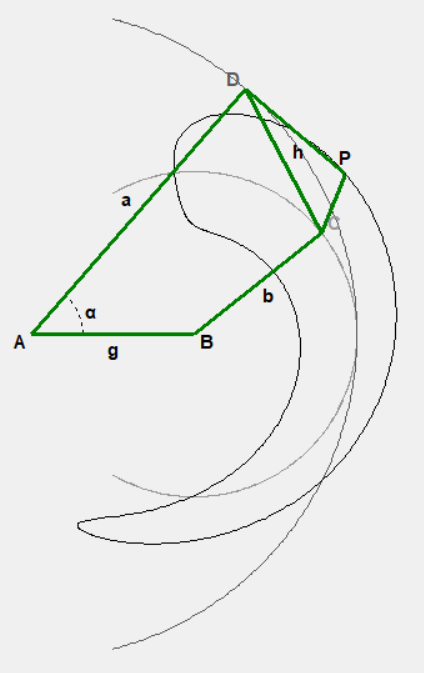
\includegraphics[width=0.5\linewidth]{./Figures/27_motion_cases/-1-1-1.png} \hfill {\tiny $T_{1,2,3} = -1.0, -1.0, -1.0$}\end{center}\end{minipage}\\
	\end{tabular}
\end{center}
\end{frame}

\subsection{Optimization problem}

\begin{frame}
\frametitle{Results \\
	\small \color{rwth-blue} Optimization problem}
	\begin{center}
		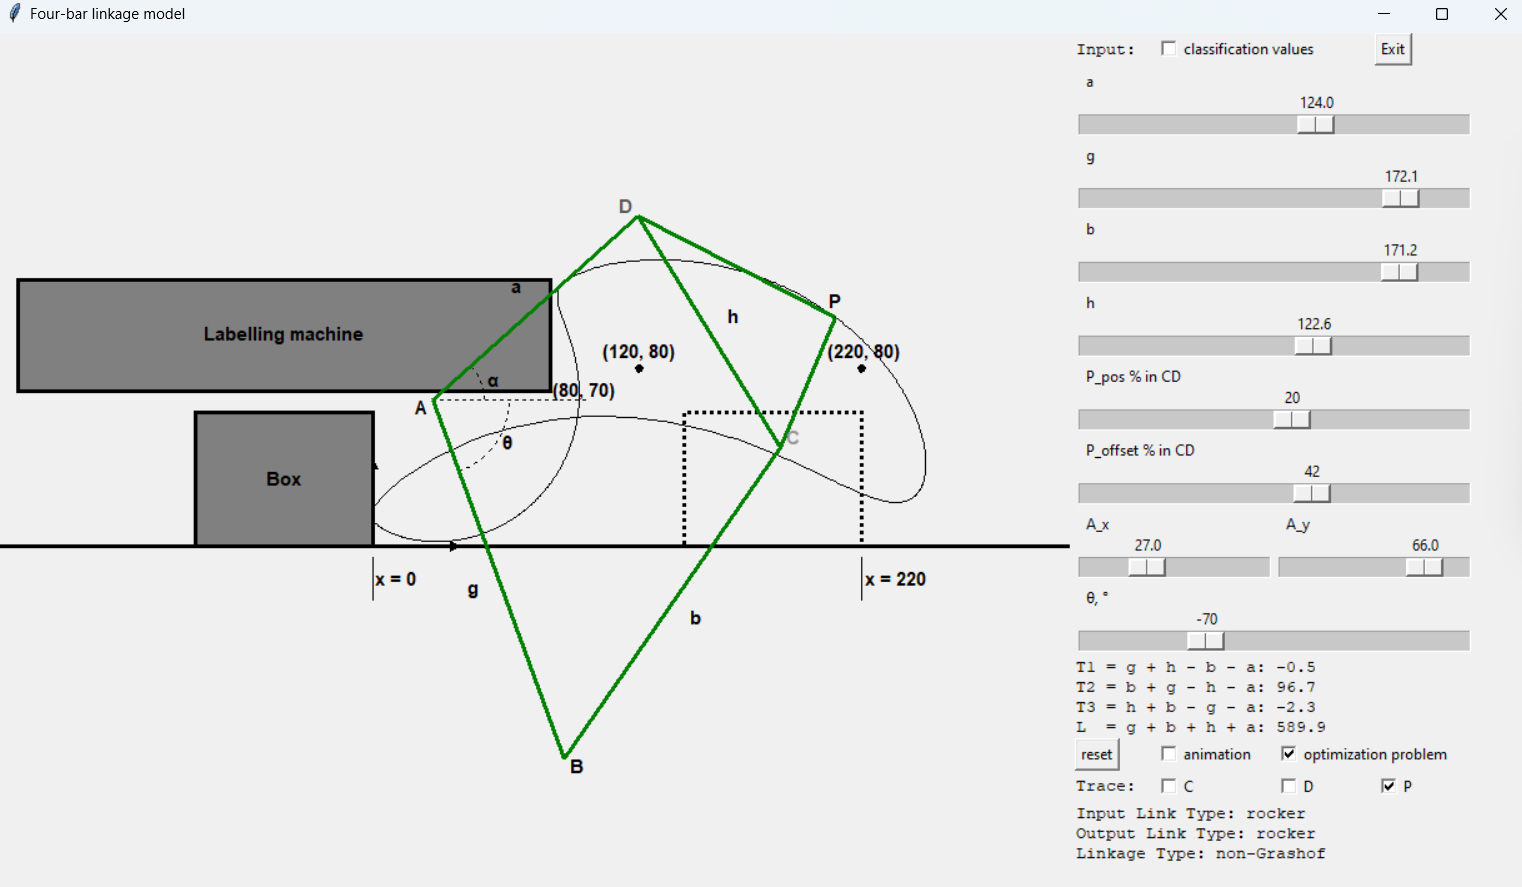
\includegraphics[width=0.8\linewidth]{./Figures/optimization_problem_solution.png}
	\end{center}
	\begin{itemize}
		\item 9 degrees of freedom (all lengths in cm):
		\begin{itemize}
			\item Length of four bars: $a = 124.0$, $b = 171.2$, $g = 172.1$, $h = 122.6$.
			\item Coupler position: $P_{pos} = 20.0 \%, P_{offset} = 42.0 \%$ of $h$.
			\item Position of point A: $A_x = 27.0$, $A_y = 66.0$.
			\item Angle of ground bar relative to horizon: $\theta = -70.0^{\circ}$
		\end{itemize}
	\end{itemize}
\end{frame}

\section{Project Management}

\begin{frame}
\frametitle{Project Management}
\end{frame}

\section{Live Software Demo}

\begin{frame}
\frametitle{Live Software Demo} 
\end{frame}

\section{Summary and Conclusion}

\begin{frame}
\frametitle{Summary and Conclusion}
\end{frame}

\begin{frame}
\frametitle{Literature}
	\begin{itemize}
		\item Cvetkovic, Ivana and Stojicevic, Misa and Popkonstantinović, Branislav and Cvetković, Dragan. (2018). Classification, geometrical and kinematic analysis of four-bar linkages. 261-266. 10.15308/Sinteza-2018-261-266.
	\end{itemize}
\end{frame}

\end{document}
